%% Seminar deck: Welfare measurements with heterogeneous agents (JEDC, 2026)
%% House style, academic register. Built from the published article's
%% abstract and structure; co-authored with Marek Weretka.
\documentclass[aspectratio=169,11pt]{beamer}
\usepackage{beamerthemeyc}
\renewcommand{\deckfootertitle}{Weretka \& Dec (2026) · Welfare measurements with heterogeneous agents · JEDC}

\begin{document}

% 1 ---------------------------------------------------------------------------
\begin{frame}[plain]
  \vspace{2mm}
  {\ttfamily\scriptsize\color{ycmuted}SEMINAR DECK · YIELDCARTOGRAPHY.COM}\\[-0.3em]
  {\color{ycrule}\rule{\textwidth}{0.5pt}}
  \vspace{4mm}

  {\fontsize{19}{23}\selectfont\bfseries\color{ycink}Welfare measurements\\with heterogeneous agents.\par}
  \vspace{6mm}
  {\small\bfseries Marek Weretka \enspace·\enspace Marcin Dec\par}
  {\footnotesize\color{ycmuted}University of Wisconsin--Madison \& FAME|GRAPE · Kozminski University \& FAME|GRAPE\par}
  \vspace{3mm}
  {\ttfamily\scriptsize\color{ycaccent}Journal of Economic Dynamics and Control, 184 (March 2026), art.\ 105252 · doi:10.1016/j.jedc.2025.105252\par}
  \vfill
  \raisebox{-1mm}{
\includegraphics[height=6mm]{kozminski_logo.png}}\hspace{5mm}
  \raisebox{-1mm}{
\includegraphics[height=6mm]{grape_logo.png}}\hspace{5mm}
  \raisebox{-1mm}{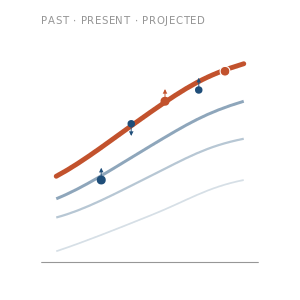
\includegraphics[height=6mm]{yc_logo.png}}
\end{frame}

% 2 ---------------------------------------------------------------------------
\begin{frame}{Motivation}
  \kicker{The missing index}
  \begin{itemize}
    \item The canonical infinite-horizon framework with heterogeneous
          consumers, standard in macroeconomics and finance, lacks a
          preference-based index that consistently quantifies the welfare
          impact of economic policies.
    \item The classic money-metric indices, equivalent and compensating
          variation, fail two consistency requirements in this setting: they
          are non-additive across sets of policies, and their predictions can
          depend on the assumed status quo or on the order in which
          alternatives are implemented.
    \item The paper delivers a positive result on when these failures become
          quantitatively negligible.
  \end{itemize}
\end{frame}

% 3 ---------------------------------------------------------------------------
\begin{frame}{Money-metric welfare indices}
  \kicker{Definitions}
  \small For consumer $i$ with lifetime utility $V_i$, wealth $w_i$ and a
  policy moving the environment from $\vartheta^0$ to $\vartheta^1$, the
  equivalent and compensating variations solve
  \[ V_i\!\left(w_i + EV_i;\,\vartheta^0\right) = V_i\!\left(w_i;\,\vartheta^1\right),
     \qquad
     V_i\!\left(w_i;\,\vartheta^0\right) = V_i\!\left(w_i - CV_i;\,\vartheta^1\right). \]
  \begin{itemize}
    \item Additivity would require the index of a bundle of policies to equal
          the sum of the indices of its elements; exact additivity fails for
          general preferences, and with it order-independence.
    \item The question is under what restrictions the money metric becomes
          approximately additive, so that policy rankings aggregate.
  \end{itemize}
\end{frame}

% 4 ---------------------------------------------------------------------------
\begin{frame}{Main result}
  \kicker{Near-additivity under patience}
  \begin{itemize}
    \item For arbitrary heterogeneous von Neumann--Morgenstern preferences
          sharing a common discount factor, the equivalent (or compensating)
          variation is nearly additive and aggregates effectively as long as
          consumers are patient.
    \item The approximation error of treating the index as additive vanishes
          as the discount factor approaches one, so for short-lived policies
          the money metric behaves as a consistent quantitative welfare
          index.
    \item Consequently, the index delivers consistent welfare predictions
          for the wide variety of short-lived policies studied in the
          macroeconomic and finance literature.
  \end{itemize}
\end{frame}

% 5 ---------------------------------------------------------------------------
\begin{frame}{Structure of the argument}
  \kicker{From example to general framework}
  \begin{itemize}
    \item A motivating example isolates the non-additivity of the money
          metric in the simplest heterogeneous-agent setting.
    \item The general framework is a small open economy with heterogeneous
          vNM consumers; the near-additivity result is established there.
    \item An approximation-in-practice section quantifies the error terms and
          shows how the index is operationalised in applied policy
          evaluation.
  \end{itemize}
\end{frame}

% 6 ---------------------------------------------------------------------------
\begin{frame}{Implications}
  \kicker{For applied policy evaluation}
  \begin{itemize}
    \item Welfare statements in heterogeneous-agent models gain a consistent
          money-metric foundation for the empirically dominant case of
          short-lived policies evaluated by patient consumers.
    \item Policy bundles can be evaluated component-wise and summed, and
          rankings are invariant to the order of implementation up to the
          quantified approximation error.
    \item The result connects the applied macro practice of reporting
          consumption-equivalent welfare numbers to an explicit preference
          foundation.
  \end{itemize}
\end{frame}

% 7 ---------------------------------------------------------------------------
\begin{frame}[plain]
  \vspace{12mm}
  {\fontsize{27}{31}\selectfont\bfseries\color{ycink}Thank you.\par}
  \vspace{6mm}
  {\normalsize\color{ycink}Marek Weretka · Marcin Dec\par}
  {\small\color{ycmuted}mdec@kozminski.edu.pl · ORCID 0000-0002-6220-8267\par}
  \vspace{5mm}
  {\ttfamily\footnotesize\color{ycaccent}%
   Weretka, M. and Dec, M. (2026). Welfare measurements with heterogeneous\\
   agents. Journal of Economic Dynamics and Control, 184, art.\ 105252.\\
   doi:10.1016/j.jedc.2025.105252 · preprint: SSRN 5335293\par}
  \vfill
  \raisebox{-1mm}{
\includegraphics[height=6mm]{kozminski_logo.png}}\hspace{5mm}
  \raisebox{-1mm}{
\includegraphics[height=6mm]{grape_logo.png}}\hspace{5mm}
  \raisebox{-1mm}{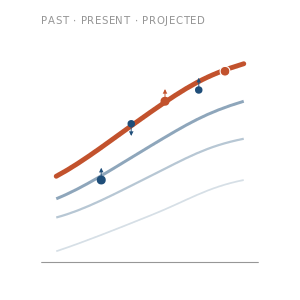
\includegraphics[height=6mm]{yc_logo.png}}
  \hfill{\ttfamily\scriptsize\color{ycmuted}yieldcartography.com/slides/welfare/}
\end{frame}

\end{document}
